\textcolor{black}{Di bagian ini, mahasiswa diharapkan mampu mendesain solusi dari permasalahan yang telah dipilih. Rancangan solusi dapat diberikan dalam bentuk skematik, diagram blok, diagram alur/\textit{flowcharts}, \textit{pseudo-codes}, dan sejenisnya.
}

Bagian ini merupakan inti dari dokumen C-251. Artinya kualitas dari dokumen C-251 ini akan ditentukan dari kualitas pada bagian ini. Peserta \textit{capstone} wajib menjelaskan secara umum desain dari sistem yang nantinya akan diimplementasikan pada \textit{Capstone} 2 di semester genap. 

Tergantung pada jenis topik yang diangkat, isi dari bagian ini dapat bervariasi. Apabila produk yang ditawarkan berupa perangkat keras, maka bagian ini pada umumnya akan berisi \textit{blueprint} umum/skematik umum perancangan hardware yang lebih bersifat blok diagram fungsional dan tidak terlalu mendetail sampai level komponen atau pun desain \textit{board} elektronis/mekanik. 

Apabila produk/luaran yang ditawarkan berupa sistem aplikasi (khususnya untuk bidang TI), bagian ini berupa DFD dan ERD berserta \textit{detail use case diagram} yang masih umum dan belum mendetail. 

Bila produk/luaran yang ditawarkan berupa program simulasi lengkap, maka pada bagian ini peserta \textit{capstone} harus menyajikan model matematika secara umum yang nantinya akan dijabarkan. Demikian pula metode atau algoritme (model matematika maupun diagram alir) yang digunakan untuk menyelesaikan permasalahan tersebut.

\section{Penyajian \textit{Flowchart}}
\titlelabel{sec:Penyajian_Flowchart}
    
    \begin{figure}[!ht]
        \centering
        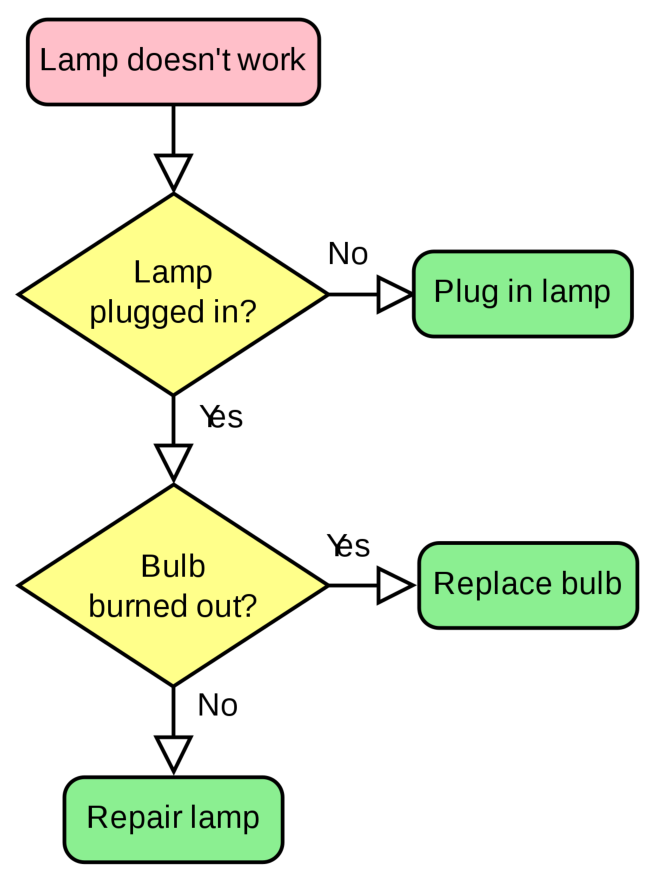
\includegraphics[scale=0.5]{Ch08_Flowchart.pdf}
        \caption{Contoh \textit{Flowchart} (Prosedur Perawatan Lampu)}
        \label{fig:Ch08_Flowchart}
    \end{figure}
    
    Peserta \textit{capstone} harus menyajikan pula model \textit{flowchart} sampai dengan proses pengujian dan verifikasi yang akan digunakan untuk menguji unjuk kerja dari desain yang dibuat. Mahasiswa bisa memilih untuk menggunakan diagram alir, diagram blok, atau algoritme. Salah satu contoh diagram alir dapat dilihat pada Gambar \ref{fig:Ch08_Flowchart}. Program simulasi lain dapat juga berupa program yang digunakan untuk menguji unjuk kerja algoritme yang digunakan untuk menjawab suatu permasalahan. Untuk bidang STL yang tidak menghasilkan perangkat keras maupun program simulasi lengkap, maka peserta \textit{capstone} harus mencantumkan model matematika yang umumnya digunakan. Misalkan, apabila problem yang diangkat berupa problem optimasi, maka peserta \textit{capstone} harus menyertakan \textit{model objective function} serta \textit{constraint} yang berkaitan, dan model algoritme optimasi yang dipakai untuk menyelesaikan problem optimasi berdasarkan sifat dari problem optimasi tersebut (misalkan : \textit{convex}/\textit{non-convex}, linear/\textit{quadratic}/fungsi lainnya, \textit{integer}).
